\documentclass[10pt,letterpaper]{book}	
% babel: Este paquete establece las reglas tipográficas (y otras reglas) para el lenguaje especificado
\usepackage[spanish]{babel} 
%  inputenc: Indicamos la codificación que se utilizará en el documento por lo general ISO-8859-1(latin1)  o utf8
\usepackage[utf8]{inputenc} 
% Para escribir comillas dobles
\usepackage[style=mexican]{csquotes}
% Para indicar secuencias de menús o combinacines de teclas
\usepackage[os=mac, mackeys=symbols]{menukeys}
% Indicamos los margenes que tendrá el documento
\usepackage[top=1in, bottom=1.25in, left=0.75in, right=0.75in]{geometry}
% Permite el uso de unidades de medida
\usepackage{siunitx}
% amsmath: Comandos extras para matemáticas (cajas para ecuaciones, etc)
\usepackage{amsmath} 
% Simbolos matematicos (por lo tanto)
\usepackage{amssymb} 
% Incluir imágenes en LaTeX
\usepackage{graphicx}
% Para poder especificar el ancho de la tabla 
\usepackage{tabularx} 
%Podemos usar el especificador [H] en las figuras para que se queden donde queramos
\usepackage{float} 
 % Permite usar etiquetas fuera de elementos flotantes (etiquetas de figuras)
\usepackage{capt-of}
% Para que las referencias sean hipervínculos a las figuras o ecuaciones y aparezcan en color
\usepackage[colorlinks=true,plainpages=true,citecolor=blue,linkcolor=blue]{hyperref}
% Utilizar un glosario
\usepackage[automake]{glossaries-extra}
\newglossaryentry{Linux}
{
  name=Linux,
  description={is a generic term referring to the family of Unix-like
               computer operating systems that use the Linux kernel},
  plural=Linuces
}

\makeglossaries
% Utilizar apéndices
\usepackage{appendix}
\renewcommand{\appendixname}{Apéndices}
\renewcommand{\appendixtocname}{Apéndices}
\renewcommand{\appendixpagename}{Apéndices} 

% Comando para poder cambiar el tamaño de las imágenes en un solo lugar
\newcommand{\GlLineWidth}{\textwidth}

%Paquete para listings-eclipse
\usepackage{rsc/pckg/lstcustom}

\author{Mauricio Ocón}
\title{Plantilla}

\begin{document}
	%Crea una hoja de portada
	\maketitle
	%Muestra el índice
	\tableofcontents	
	% Para que aparezcan las referencias sin citar
	\nocite{*}	
	
	%%%%%%% Capítulos %%%%%%%% 		
	\chapter{Introducción}

Lorem ipsum dolor sit amet, consectetur adipiscing elit. Nam viverra sagittis sapien, mollis ornare dolor. Donec fermentum, justo vitae tristique accumsan, urna ex dignissim risus, vitae tempor ante arcu condimentum turpis. Vestibulum tincidunt nulla nec lacus laoreet porttitor. Donec placerat congue mi, cursus dictum dolor viverra vitae. Phasellus venenatis, sapien in congue ornare, augue quam rutrum justo, vel molestie arcu metus luctus urna. Praesent egestas et leo vel ullamcorper. Etiam porta lectus dolor, vitae commodo arcu posuere in. Duis cursus suscipit lacus et tempus. Ut aliquet porttitor tortor in accumsan. Fusce pretium erat non ante tempor ultrices. Donec lorem justo, tincidunt ac finibus sit amet, tempor et dui. Fusce fermentum tempor nisl in blandit. Nam eu neque accumsan, varius tortor in, dictum justo. Ut rutrum tempus tellus, at sollicitudin velit ullamcorper non. In vel velit diam. Sed eu lectus iaculis, porta nisi sit amet, faucibus odio.

	\section{Sección 1}
	
	Quisque rhoncus sit amet ex id porttitor. Aenean faucibus lectus at leo commodo feugiat. Mauris blandit ipsum non accumsan euismod. Cras nisi nunc, ultricies vel tellus non, ultrices iaculis mauris. Phasellus lorem lorem, cursus nec enim in, porta interdum arcu. Fusce ut imperdiet odio. Sed imperdiet eget enim at pellentesque.
	
	\begin{figure}[H]
		\begin{center}
			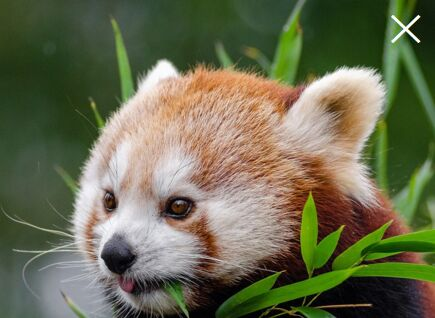
\includegraphics[width = 0.8\imageWidth]{rsc/img/TestImage}
			\captionof{figure}{\label{fig:testImgRef}Pie de imagen} 
		\end{center} 
	\end{figure}
	
	Quisque rhoncus sit amet ex id porttitor. Aenean faucibus lectus at leo commodo feugiat. Mauris blandit ipsum non accumsan euismod. Cras nisi nunc, ultricies vel tellus non, ultrices iaculis mauris. Phasellus lorem lorem, cursus nec enim in, porta interdum arcu. Fusce ut imperdiet odio. Sed imperdiet eget enim at pellentesque.
	
	Quisque rhoncus sit amet ex id porttitor. Aenean faucibus lectus at leo commodo feugiat. Mauris blandit ipsum non accumsan euismod. Cras nisi nunc, ultricies vel tellus non, ultrices iaculis mauris. Phasellus lorem lorem, cursus nec enim in, porta interdum arcu. Fusce ut imperdiet odio. Sed imperdiet eget enim at pellentesque.\cite{IEEEreferencias:Ref1}
	
	Quisque rhoncus sit amet ex id porttitor. Aenean faucibus lectus at leo commodo feugiat. Mauris blandit ipsum non accumsan euismod. Cras nisi nunc, ultricies vel tellus non, ultrices iaculis mauris. Phasellus lorem lorem, cursus nec enim in, porta interdum arcu. Fusce ut imperdiet odio. Sed imperdiet eget enim at pellentesque.\gls{Linux}
	
	
	
	\section{Sección 2}
	
	Vestibulum sollicitudin imperdiet nisl. Nullam eget nisi nunc. Quisque eget accumsan lorem, nec interdum neque. Pellentesque habitant morbi tristique senectus et netus et malesuada fames ac turpis egestas. Vestibulum ante ipsum primis in faucibus orci luctus et ultrices posuere cubilia Curae; Nullam at metus dignissim, euismod diam in, maximus sem. Sed semper rhoncus lectus eu tempor.
	
	Vestibulum sollicitudin imperdiet nisl. Nullam eget nisi nunc. Quisque eget accumsan lorem, nec interdum neque. Pellentesque habitant morbi tristique senectus et netus et malesuada fames ac turpis egestas. Vestibulum ante ipsum primis in faucibus orci luctus et ultrices posuere cubilia Curae; Nullam at metus dignissim, euismod diam in, maximus sem. Sed semper rhoncus lectus eu tempor.
	
	Vestibulum sollicitudin imperdiet nisl. Nullam eget nisi nunc. Quisque eget accumsan lorem, nec interdum neque. Pellentesque habitant morbi tristique senectus et netus et malesuada fames ac turpis egestas. Vestibulum ante ipsum primis in faucibus orci luctus et ultrices posuere cubilia Curae; Nullam at metus dignissim, euismod diam in, maximus sem. Sed semper rhoncus lectus eu tempor.
	
	Vestibulum sollicitudin imperdiet nisl. Nullam eget nisi nunc. Quisque eget accumsan lorem, nec interdum neque. Pellentesque habitant morbi tristique senectus et netus et malesuada fames ac turpis egestas. Vestibulum ante ipsum primis in faucibus orci luctus et ultrices posuere cubilia Curae; Nullam at metus dignissim, euismod diam in, maximus sem. Sed semper rhoncus lectus eu tempor.
	
	\section{Sección 3}
	
	Phasellus bibendum dignissim efficitur. Vestibulum venenatis leo in lorem blandit dignissim. Praesent scelerisque dapibus lectus vel efficitur. Fusce tristique nulla at tempor eleifend. Vivamus ullamcorper volutpat lorem. Integer sodales molestie cursus. Aliquam felis mi, ultricies nec ante a, tincidunt semper nulla. In convallis finibus nibh id ultrices.

	\section{Sección 4}
	Quisque ligula ex, semper eu tristique sit amet, accumsan vitae eros. Proin sodales hendrerit metus sit amet tincidunt. Etiam dictum cursus tellus id malesuada. Integer accumsan augue eu lectus consectetur, vel interdum turpis posuere. Pellentesque pellentesque lacinia enim, semper consectetur sem lacinia in. Etiam bibendum tristique justo ac blandit. Curabitur vitae dapibus odio, tempus ornare dolor. Maecenas dui urna, luctus at auctor at, tincidunt non eros. Proin euismod, lacus nec faucibus congue, orci magna vulputate est, quis tempus orci urna eget justo. Nulla a placerat turpis.

	
	\chapter{Introducción}

Lorem ipsum dolor sit amet, consectetur adipiscing elit. Nam viverra sagittis sapien, mollis ornare dolor. Donec fermentum, justo vitae tristique accumsan, urna ex dignissim risus, vitae tempor ante arcu condimentum turpis. Vestibulum tincidunt nulla nec lacus laoreet porttitor. Donec placerat congue mi, cursus dictum dolor viverra vitae. Phasellus venenatis, sapien in congue ornare, augue quam rutrum justo, vel molestie arcu metus luctus urna. Praesent egestas et leo vel ullamcorper. Etiam porta lectus dolor, vitae commodo arcu posuere in. Duis cursus suscipit lacus et tempus. Ut aliquet porttitor tortor in accumsan. Fusce pretium erat non ante tempor ultrices. Donec lorem justo, tincidunt ac finibus sit amet, tempor et dui. Fusce fermentum tempor nisl in blandit. Nam eu neque accumsan, varius tortor in, dictum justo. Ut rutrum tempus tellus, at sollicitudin velit ullamcorper non. In vel velit diam. Sed eu lectus iaculis, porta nisi sit amet, faucibus odio.

	\section{Sección 1}
	
	Quisque rhoncus sit amet ex id porttitor. Aenean faucibus lectus at leo commodo feugiat. Mauris blandit ipsum non accumsan euismod. Cras nisi nunc, ultricies vel tellus non, ultrices iaculis mauris. Phasellus lorem lorem, cursus nec enim in, porta interdum arcu. Fusce ut imperdiet odio. Sed imperdiet eget enim at pellentesque.
	
	\section{Sección 2}
	
	Vestibulum sollicitudin imperdiet nisl. Nullam eget nisi nunc. Quisque eget accumsan lorem, nec interdum neque. Pellentesque habitant morbi tristique senectus et netus et malesuada fames ac turpis egestas. Vestibulum ante ipsum primis in faucibus orci luctus et ultrices posuere cubilia Curae; Nullam at metus dignissim, euismod diam in, maximus sem. Sed semper rhoncus lectus eu tempor.
	
	\section{Sección 3}
	
	Phasellus bibendum dignissim efficitur. Vestibulum venenatis leo in lorem blandit dignissim. Praesent scelerisque dapibus lectus vel efficitur. Fusce tristique nulla at tempor eleifend. Vivamus ullamcorper volutpat lorem. Integer sodales molestie cursus. Aliquam felis mi, ultricies nec ante a, tincidunt semper nulla. In convallis finibus nibh id ultrices.

	\section{Sección 4}
	Quisque ligula ex, semper eu tristique sit amet, accumsan vitae eros. Proin sodales hendrerit metus sit amet tincidunt. Etiam dictum cursus tellus id malesuada. Integer accumsan augue eu lectus consectetur, vel interdum turpis posuere. Pellentesque pellentesque lacinia enim, semper consectetur sem lacinia in. Etiam bibendum tristique justo ac blandit. Curabitur vitae dapibus odio, tempus ornare dolor. Maecenas dui urna, luctus at auctor at, tincidunt non eros. Proin euismod, lacus nec faucibus congue, orci magna vulputate est, quis tempus orci urna eget justo. Nulla a placerat turpis.

	
	\chapter{Introducción}

Lorem ipsum dolor sit amet, consectetur adipiscing elit. Nam viverra sagittis sapien, mollis ornare dolor. Donec fermentum, justo vitae tristique accumsan, urna ex dignissim risus, vitae tempor ante arcu condimentum turpis. Vestibulum tincidunt nulla nec lacus laoreet porttitor. Donec placerat congue mi, cursus dictum dolor viverra vitae. Phasellus venenatis, sapien in congue ornare, augue quam rutrum justo, vel molestie arcu metus luctus urna. Praesent egestas et leo vel ullamcorper. Etiam porta lectus dolor, vitae commodo arcu posuere in. Duis cursus suscipit lacus et tempus. Ut aliquet porttitor tortor in accumsan. Fusce pretium erat non ante tempor ultrices. Donec lorem justo, tincidunt ac finibus sit amet, tempor et dui. Fusce fermentum tempor nisl in blandit. Nam eu neque accumsan, varius tortor in, dictum justo. Ut rutrum tempus tellus, at sollicitudin velit ullamcorper non. In vel velit diam. Sed eu lectus iaculis, porta nisi sit amet, faucibus odio.

	\section{Sección 1}
	
	Quisque rhoncus sit amet ex id porttitor. Aenean faucibus lectus at leo commodo feugiat. Mauris blandit ipsum non accumsan euismod. Cras nisi nunc, ultricies vel tellus non, ultrices iaculis mauris. Phasellus lorem lorem, cursus nec enim in, porta interdum arcu. Fusce ut imperdiet odio. Sed imperdiet eget enim at pellentesque.
	
	\section{Sección 2}
	
	Vestibulum sollicitudin imperdiet nisl. Nullam eget nisi nunc. Quisque eget accumsan lorem, nec interdum neque. Pellentesque habitant morbi tristique senectus et netus et malesuada fames ac turpis egestas. Vestibulum ante ipsum primis in faucibus orci luctus et ultrices posuere cubilia Curae; Nullam at metus dignissim, euismod diam in, maximus sem. Sed semper rhoncus lectus eu tempor.
	
	\section{Sección 3}
	
	Phasellus bibendum dignissim efficitur. Vestibulum venenatis leo in lorem blandit dignissim. Praesent scelerisque dapibus lectus vel efficitur. Fusce tristique nulla at tempor eleifend. Vivamus ullamcorper volutpat lorem. Integer sodales molestie cursus. Aliquam felis mi, ultricies nec ante a, tincidunt semper nulla. In convallis finibus nibh id ultrices.

	\section{Sección 4}
	Quisque ligula ex, semper eu tristique sit amet, accumsan vitae eros. Proin sodales hendrerit metus sit amet tincidunt. Etiam dictum cursus tellus id malesuada. Integer accumsan augue eu lectus consectetur, vel interdum turpis posuere. Pellentesque pellentesque lacinia enim, semper consectetur sem lacinia in. Etiam bibendum tristique justo ac blandit. Curabitur vitae dapibus odio, tempus ornare dolor. Maecenas dui urna, luctus at auctor at, tincidunt non eros. Proin euismod, lacus nec faucibus congue, orci magna vulputate est, quis tempus orci urna eget justo. Nulla a placerat turpis.

	%%%%%%%%%%%%%%%%%%%%%%%%%%
	
	
	%%%%%%% Apéndices %%%%%%%%   	
	\appendix   
	\clearpage % o \cleardoublepage
	\addappheadtotoc 
	\appendixpage 
	%%%%%%%%%%%%%%%%%%%%%%%%%%
	
	%%%%%%% Anexos %%%%%%%% 
	\chapter{Anexos 1}

Lorem ipsum dolor sit amet, consectetur adipiscing elit. Nam viverra sagittis sapien, mollis ornare dolor. Donec fermentum, justo vitae tristique accumsan, urna ex dignissim risus, vitae tempor ante arcu condimentum turpis. Vestibulum tincidunt nulla nec lacus laoreet porttitor. Donec placerat congue mi, cursus dictum dolor viverra vitae. Phasellus venenatis, sapien in congue ornare, augue quam rutrum justo, vel molestie arcu metus luctus urna. Praesent egestas et leo vel ullamcorper. Etiam porta lectus dolor, vitae commodo arcu posuere in. Duis cursus suscipit lacus et tempus. Ut aliquet porttitor tortor in accumsan. Fusce pretium erat non ante tempor ultrices. Donec lorem justo, tincidunt ac finibus sit amet, tempor et dui. Fusce fermentum tempor nisl in blandit. Nam eu neque accumsan, varius tortor in, dictum justo. Ut rutrum tempus tellus, at sollicitudin velit ullamcorper non. In vel velit diam. Sed eu lectus iaculis, porta nisi sit amet, faucibus odio.

	\section{Sección 1}
	
	Quisque rhoncus sit amet ex id porttitor. Aenean faucibus lectus at leo commodo feugiat. Mauris blandit ipsum non accumsan euismod. Cras nisi nunc, ultricies vel tellus non, ultrices iaculis mauris. Phasellus lorem lorem, cursus nec enim in, porta interdum arcu. Fusce ut imperdiet odio. Sed imperdiet eget enim at pellentesque.
	
	\section{Sección 2}
	
	Vestibulum sollicitudin imperdiet nisl. Nullam eget nisi nunc. Quisque eget accumsan lorem, nec interdum neque. Pellentesque habitant morbi tristique senectus et netus et malesuada fames ac turpis egestas. Vestibulum ante ipsum primis in faucibus orci luctus et ultrices posuere cubilia Curae; Nullam at metus dignissim, euismod diam in, maximus sem. Sed semper rhoncus lectus eu tempor.
	
	\section{Sección 3}
	
	Phasellus bibendum dignissim efficitur. Vestibulum venenatis leo in lorem blandit dignissim. Praesent scelerisque dapibus lectus vel efficitur. Fusce tristique nulla at tempor eleifend. Vivamus ullamcorper volutpat lorem. Integer sodales molestie cursus. Aliquam felis mi, ultricies nec ante a, tincidunt semper nulla. In convallis finibus nibh id ultrices.

	\section{Sección 4}
	Quisque ligula ex, semper eu tristique sit amet, accumsan vitae eros. Proin sodales hendrerit metus sit amet tincidunt. Etiam dictum cursus tellus id malesuada. Integer accumsan augue eu lectus consectetur, vel interdum turpis posuere. Pellentesque pellentesque lacinia enim, semper consectetur sem lacinia in. Etiam bibendum tristique justo ac blandit. Curabitur vitae dapibus odio, tempus ornare dolor. Maecenas dui urna, luctus at auctor at, tincidunt non eros. Proin euismod, lacus nec faucibus congue, orci magna vulputate est, quis tempus orci urna eget justo. Nulla a placerat turpis.

	
	\chapter{Anexos 2}

Lorem ipsum dolor sit amet, consectetur adipiscing elit. Nam viverra sagittis sapien, mollis ornare dolor. Donec fermentum, justo vitae tristique accumsan, urna ex dignissim risus, vitae tempor ante arcu condimentum turpis. Vestibulum tincidunt nulla nec lacus laoreet porttitor. Donec placerat congue mi, cursus dictum dolor viverra vitae. Phasellus venenatis, sapien in congue ornare, augue quam rutrum justo, vel molestie arcu metus luctus urna. Praesent egestas et leo vel ullamcorper. Etiam porta lectus dolor, vitae commodo arcu posuere in. Duis cursus suscipit lacus et tempus. Ut aliquet porttitor tortor in accumsan. Fusce pretium erat non ante tempor ultrices. Donec lorem justo, tincidunt ac finibus sit amet, tempor et dui. Fusce fermentum tempor nisl in blandit. Nam eu neque accumsan, varius tortor in, dictum justo. Ut rutrum tempus tellus, at sollicitudin velit ullamcorper non. In vel velit diam. Sed eu lectus iaculis, porta nisi sit amet, faucibus odio.

	\section{Sección 1}
	
	Quisque rhoncus sit amet ex id porttitor. Aenean faucibus lectus at leo commodo feugiat. Mauris blandit ipsum non accumsan euismod. Cras nisi nunc, ultricies vel tellus non, ultrices iaculis mauris. Phasellus lorem lorem, cursus nec enim in, porta interdum arcu. Fusce ut imperdiet odio. Sed imperdiet eget enim at pellentesque.
	
	\section{Sección 2}
	
	Vestibulum sollicitudin imperdiet nisl. Nullam eget nisi nunc. Quisque eget accumsan lorem, nec interdum neque. Pellentesque habitant morbi tristique senectus et netus et malesuada fames ac turpis egestas. Vestibulum ante ipsum primis in faucibus orci luctus et ultrices posuere cubilia Curae; Nullam at metus dignissim, euismod diam in, maximus sem. Sed semper rhoncus lectus eu tempor.
	
	\section{Sección 3}
	
	Phasellus bibendum dignissim efficitur. Vestibulum venenatis leo in lorem blandit dignissim. Praesent scelerisque dapibus lectus vel efficitur. Fusce tristique nulla at tempor eleifend. Vivamus ullamcorper volutpat lorem. Integer sodales molestie cursus. Aliquam felis mi, ultricies nec ante a, tincidunt semper nulla. In convallis finibus nibh id ultrices.

	\section{Sección 4}
	Quisque ligula ex, semper eu tristique sit amet, accumsan vitae eros. Proin sodales hendrerit metus sit amet tincidunt. Etiam dictum cursus tellus id malesuada. Integer accumsan augue eu lectus consectetur, vel interdum turpis posuere. Pellentesque pellentesque lacinia enim, semper consectetur sem lacinia in. Etiam bibendum tristique justo ac blandit. Curabitur vitae dapibus odio, tempus ornare dolor. Maecenas dui urna, luctus at auctor at, tincidunt non eros. Proin euismod, lacus nec faucibus congue, orci magna vulputate est, quis tempus orci urna eget justo. Nulla a placerat turpis.

	%%%%%%%%%%%%%%%%%%%%%%%%%%
	
	\printglossaries
	
	%%%%%%% Bibliografía %%%%%%%%
	\bibliographystyle{bst/IEEEtran.bst} 
	\addcontentsline{toc}{chapter}{Referencias}  
	\bibliography{bib/IEEEabrv,bib/IEEEreferences.bib} 
	%%%%%%%%%%%%%%%%%%%%%%%%%%%%%
	
\end{document}